\documentclass[11pt,a4paper]{article}
% Supplementary material of main.tex. Build after make_tables.py: latexmk -pdf supplement.tex (then main.tex, which
% reads supplement.aux through xr for the S-numbered cross-references).
\usepackage[margin=2.5cm]{geometry}
\usepackage[T1]{fontenc}
\usepackage{amsmath,amssymb,amsthm}
\usepackage{booktabs,graphicx,xcolor}
\usepackage{algorithm}
\usepackage[noend]{algpseudocode}
\usepackage{natbib}
\usepackage{xr}
\usepackage[colorlinks=true,linkcolor=blue!50!black,citecolor=blue!50!black,urlcolor=blue!50!black]{hyperref}
\usepackage[capitalise,nameinlink]{cleveref}
\usepackage{float}
\usepackage[section]{placeins}
\externaldocument[M-]{main}

\renewcommand{\thesection}{S\arabic{section}}
\renewcommand{\thetable}{S\arabic{table}}
\renewcommand{\thefigure}{S\arabic{figure}}
\renewcommand{\theequation}{S\arabic{equation}}
\renewcommand{\thealgorithm}{S\arabic{algorithm}}
\crefname{algorithm}{Algorithm}{Algorithms}
\crefname{section}{Section}{Sections}

\newcommand{\todo}[1]{\textcolor{red!70!black}{\textbf{[TODO:} #1\textbf{]}}}
\newcommand{\pend}{\textcolor{red!70!black}{[pending]}}
\newcommand{\R}{\mathbb{R}}
\newcommand{\B}{\mathcal{B}}
\newcommand{\I}{\mathcal{I}}
\newcommand{\A}{\mathcal{A}}
\newcommand{\sig}{\sigma}
\DeclareMathOperator*{\argmax}{arg\,max}

\title{Supplementary material for\\ ``Constructive neural networks with certified partial monotonicity for binary
classification''}
\author{Ghabriel A. G. de Sá, Cristiano H. O. Fontes, Marcelo Embiruçu}
\date{}

\begin{document}
\maketitle

\noindent Section, equation, table, figure and algorithm numbers without the prefix S refer to the main article.

% =====================================================================================================
\section{Proofs}\label{sup:proofs}

\paragraph{\Cref{M-lem:gain}}
By the chain rule,
\[
\frac{\partial p_\theta}{\partial x_i}=\sig'(z_o)\,\frac{\partial z_o}{\partial x_i},\qquad
\frac{\partial z_o}{\partial x_i}=\sum_j v_j\sig'(z_j)W_{ji}.
\]
Multiplying by $s_i$ gives $s_ig_i=\sig'(z_o)\sum_j s_iv_jW_{ji}\sig'(z_j)=\sig'(z_o)h_i$, and $\sig'(z_o)>0$.

\paragraph{\Cref{M-prop:sign}}
If $c_{ij}\ge0$ for all $j$, then $h_i(x)=\sum_jc_{ij}\sig'(z_j(x))\ge0$ for every $x\in\R^p$ because $\sig'>0$;
conclude with \cref{M-lem:gain} and \cref{M-def:mono}.

\paragraph{\Cref{M-thm:ua}}
Let $F=\sig^{-1}\circ f$. Since $f(\B)$ is a compact subset of $(0,1)$, $F$ is continuous and, $\sig^{-1}$ being
increasing, $s$-monotone. \emph{Extension.} Let $\pi:\R^p\to\B$ clip every coordinate to $[0,1]$ and
$\tilde F=F\circ\pi$; $\tilde F$ is continuous, bounded and $s$-monotone on $\R^p$, because increasing $x_i$ increases
$\pi(x)_i$ or leaves it unchanged and does not affect the other coordinates. \emph{Smoothing.} Let $\phi_\delta\ge0$ be a
smooth mollifier supported in the ball of radius $\delta$ with $\int\phi_\delta=1$, and $F_\delta=\tilde F*\phi_\delta$.
Then $F_\delta\in C^\infty$, and for $t\ge0$,
$s_i\bigl(F_\delta(x+te_i)-F_\delta(x)\bigr)=\int\phi_\delta(y)\,s_i\bigl(\tilde F(x-y+te_i)-\tilde F(x-y)\bigr)dy\ge0$, so
$s_i\,\partial_iF_\delta\ge0$; by uniform continuity of $\tilde F$ on a neighbourhood of $\B$,
$\sup_\B|F_\delta-F|\to0$ as $\delta\to0$. \emph{Margin.} Let $\eta>0$ and
$H=F_\delta+\eta\sum_{i\in\I}s_ix_i$; then $s_i\partial_iH\ge\eta$ on $\B$ for $i\in\I$. \emph{Approximation.} The
logistic function is non-constant and has bounded derivatives of every order, so by \citet[Theorem 3]{Hornik1991} functions of the form
$z_o(x)=\sum_jv_j\sig(w_j^\top x+b_j)+c$ are dense in $C^1$ on compact sets: there is $z_o$ with
$\sup_\B|z_o-H|<\eta$ and $\sup_\B|\partial_iz_o-\partial_iH|<\eta/2$ for $i\in\I$. Hence
$s_i\partial_iz_o>\eta/2$ on $\B$, and $p_\theta=\sig(z_o)$ has $s_ig_i=\sig'(z_o)s_i\partial_iz_o>0$; by
\cref{M-lem:gain}, $h_i=s_i\partial_iz_o>\eta/2$, so the minimum of $h_i$ on the compact set $\B$ is positive.
\emph{Error.} Since $\sig$ is $\tfrac14$-Lipschitz,
$\sup_\B|p_\theta-f|\le\tfrac14\bigl(\sup_\B|z_o-H|+\eta\,|\I|+\sup_\B|F_\delta-F|\bigr)<\varepsilon$ for $\eta$ and
$\delta$ small enough. Finite termination of \cref{alg:bb} follows from \cref{M-prop:term}.

\paragraph{Bounds}
(a) For $x\in Q$, $w_j^\top x+b_j=w_j^\top m+b_j+w_j^\top(x-m)$ with $|w_j^\top(x-m)|\le|w_j|^\top r$, attained at a
vertex, so $z_j(Q)=[\alpha_j,\beta_j]$. Since $\sig'$ is even and unimodal with its maximum at $0$, its minimum over an
interval is attained at an endpoint and its maximum at the point of the interval closest to $0$; summing
$c_j\sig'(z_j(x))\ge c_j\underline d_j$ ($c_j\ge0$) and $\ge c_j\overline d_j$ ($c_j<0$) gives the first term of
\eqref{M-eq:lbx}. (b) The range of $\sig''$ on $[\alpha_j,\beta_j]$ is attained at the endpoints or at $\pm t^\ast$, so
$[\underline e_j,\overline e_j]$ encloses $\sig''(z_j(x))$ for $x\in Q$, and interval arithmetic on
$\sum_jc_jW_{jd}\sig''(z_j)$ encloses $\partial_dh$ on $Q$. The mean value theorem gives
$h(x)\ge h(m)-\sum_d|x_d-m_d|\sup_Q|\partial_dh|\ge h(m)-\sum_dr_d\max\{|G^-_d|,|G^+_d|\}$. (c) If $G^-_d>0$, $h$ is
increasing in $x_d$ on $Q$, so $\min_Qh$ is attained on the face $x_d=l_d$ (symmetrically for $G^+_d<0$); replacing $Q$
by that face does not change $\min_Qh$. (d) $\varphi$ is a sum of functions of one coordinate each, so its minimum over a
product of intervals is the sum of the one-dimensional minima, given by the unimodality of $\sig'$ as in (a).

\paragraph{\Cref{M-thm:sound}}
Every point of $\B$ belongs to a box of the initial list, and every box is either split into two boxes that cover it,
reduced to a face on which $h$ attains its minimum over the box (c), or discarded. A box is discarded only if
$L(Q)\ge0$, which by (a)--(b) implies $h\ge0$ on $Q$; or, in pre-activation space, if $\min_R\varphi\ge0$, which implies
$h(x)=\varphi(Wx+b)\ge0$ for every $x$ with $Wx+b\in R$ (d); or if $R$ does not meet $Z$, in which case no $x\in\B$ maps
into $R$. If the search ends with an empty list, $\min_\B h_i\ge0$ and, by \cref{M-lem:gain}, $s_ig_i\ge0$ on $\B$. A
counterexample is returned only after evaluating $h(\hat x)<0$ at a point $\hat x\in\B$ (the centre of a sub-box of $\B$,
or the solution of a linear program with bounds $0\le x\le1$).

\paragraph{\Cref{M-prop:term}}
Inputs with $\sum_j|c_jW_{jd}|=0$ do not affect $h$ and are never split; along every other coordinate the splitting rule
halves a coordinate of largest weighted width, so under breadth-first processing the radius of every box at depth $k$
tends to zero with $k$. Let $\Gamma=\frac{\sqrt3}{18}\sum_d\sum_j|c_jW_{jd}|$, an upper bound of
$\max\{|G^-_d|,|G^+_d|\}$ summed over $d$. If $\min_\B h=\delta>0$, the mean-value term of \eqref{M-eq:lbx} is at least
$\delta-\Gamma\max_dr_d$, positive once $\max_dr_d<\delta/\Gamma$, so every branch is discarded at finite depth. If
$\min_\B h<0$, continuity gives a box $Q^\ast\subseteq\B$ on which $h<0$; boxes that contain a point of $Q^\ast$ are never
discarded, and at finite depth one of them lies inside $Q^\ast$, whose centre is then a counterexample. The monotonicity
test only replaces boxes by faces that contain their minimisers and does not affect either argument.

% =====================================================================================================
\section{Branch-and-bound certificate}\label{sup:bb}
\Cref{alg:bb} decides, for one constrained input $i$ at a time, whether $\min_\B h_i\ge0$ (Section~\ref{M-sec:certificate});
write $c_j=c_{ij}$ and $h=h_i$. The bounds rely on elementary facts: $\sig'$ is even, increasing on $(-\infty,0]$ and
decreasing on $[0,\infty)$; $\sig''$ is odd, with maximum $\sqrt3/18$ at $-t^\ast$ and minimum $-\sqrt3/18$ at $t^\ast$,
$t^\ast=\ln(2+\sqrt3)$, and monotone between these points and on either side of them. On a box $Q=[l,u]$ with centre $m$
and radius $r$, $[\alpha_j,\beta_j]$, $\underline d_j$ and $\overline d_j$ are as in Section~\ref{M-sec:certificate},
$[\underline e_j,\overline e_j]$ is the range of $\sig''$ on $[\alpha_j,\beta_j]$, and interval arithmetic on
$\partial h/\partial x_d=\sum_jc_jW_{jd}\sig''(z_j)$ gives the enclosure $[G^-_d,G^+_d]$. $L(Q)$ denotes the right-hand
side of Eq.~\eqref{M-eq:lbx}. In pre-activation space the search starts from the bounding box of the zonotope
$Z=\{Wx+b:x\in\B\}$, splits the box with the most negative bound first and, for boxes that meet $Z$, evaluates $h$ at the
solution of the linear program (minimising the linearisation of $\varphi$ at the centre of $R$), which yields
counterexamples. The certificate is run once per constrained input on the final network, with budgets of
$2\times10^5$ boxes in input space and 3000 linear programs in pre-activation space.

\begin{algorithm*}[!tbp]
\caption{Branch-and-bound certificate for input $i$ ($h=h_i$).}\label{alg:bb}
\begin{algorithmic}[1]
\If{$c_j\ge0$ for all $j$} \Return \textsc{certified} \EndIf
\State $\mathcal{Q}\gets\{\B\}$ \Comment{input space; pre-activation space when $n<p$ and the input-space search exhausts $N/4$ boxes}
\While{$\mathcal{Q}\neq\emptyset$}
  \State remove a box $Q$ from $\mathcal{Q}$; apply the monotonicity test to $Q$
  \If{$L(Q)\ge0$ (\eqref{M-eq:lbx}; \eqref{M-eq:lbz} in pre-activation space) \textbf{or} $Q$ does not meet $Z$} \textbf{continue} \EndIf
  \State $\hat x\gets$ centre of $Q$ (pre-activation space: point returned by the linear program)
  \If{$h(\hat x)<0$} \Return \textsc{counterexample} $\hat x$ \EndIf
  \If{more than $N$ boxes processed} \Return \textsc{unknown} \EndIf
  \State split $Q$ in half along $\argmax_d (u_d-l_d)\max\{|G^-_d|,|G^+_d|\}$ (pre-activation space: $\argmax_j(\zeta^u_j-\zeta^l_j)|c_j|$); add both halves to $\mathcal{Q}$
\EndWhile
\State \Return \textsc{certified}
\end{algorithmic}
\end{algorithm*}

\IfFileExists{tables/cert_bench.tex}{\begin{table}[t]\centering\small
\caption{Ablation of the certificate (\cref{alg:bb}) on 168 SLFNs (56 of each kind: seven real datasets, $n\in\{2,4,8,16\}$, two seeds), with the same budget of $2\times10^5$ boxes. Outcome shares (\%) and time per network (median and 90th percentile, ms). Dense sampling ($5\times10^4$ points) finds violations in 71\%, 20\% and 0\% of the unconstrained, mean-constrained and cegis networks; no certified network has a sampled violation.}
\label{tab:certbench}
\resizebox{\textwidth}{!}{\begin{tabular}{llrrrrr}\toprule
Networks & Bounds & certified & counterex. & unknown & median & p90 \\\midrule
unconstrained & natural interval extension & 28.6 & 71.4 & 0.0 & 0.4 & 5 \\
 & + mean-value form & 28.6 & 71.4 & 0.0 & 0.3 & 5 \\
 & + monotonicity test & 28.6 & 71.4 & 0.0 & 0.6 & 8 \\
 & + pre-activation space & 28.6 & 71.4 & 0.0 & 0.5 & 8 \\
\midrule
mean constraint & natural interval extension & 80.4 & 17.9 & 1.8 & 0.1 & 8 \\
 & + mean-value form & 80.4 & 17.9 & 1.8 & 0.1 & 7 \\
 & + monotonicity test & 80.4 & 19.6 & 0.0 & 0.1 & 7 \\
 & + pre-activation space & 80.4 & 19.6 & 0.0 & 0.1 & 7 \\
\midrule
cegis step & natural interval extension & 75.0 & 0.0 & 25.0 & 0.1 & 707 \\
 & + mean-value form & 85.7 & 0.0 & 14.3 & 0.1 & 626 \\
 & + monotonicity test & 89.3 & 0.0 & 10.7 & 0.1 & 686 \\
 & + pre-activation space & 96.4 & 0.0 & 3.6 & 0.0 & 338 \\
\bottomrule\end{tabular}}\end{table}}{}

% =====================================================================================================
\section{Capacity of the constraint families}\label{sup:capacity}
\Cref{fig:capacity} repeats the comparison of Fig.~\ref{M-fig:surfaces} over the number of hidden units.

\begin{figure*}[!tbp]\centering
\IfFileExists{figures/fig_capacity.pdf}{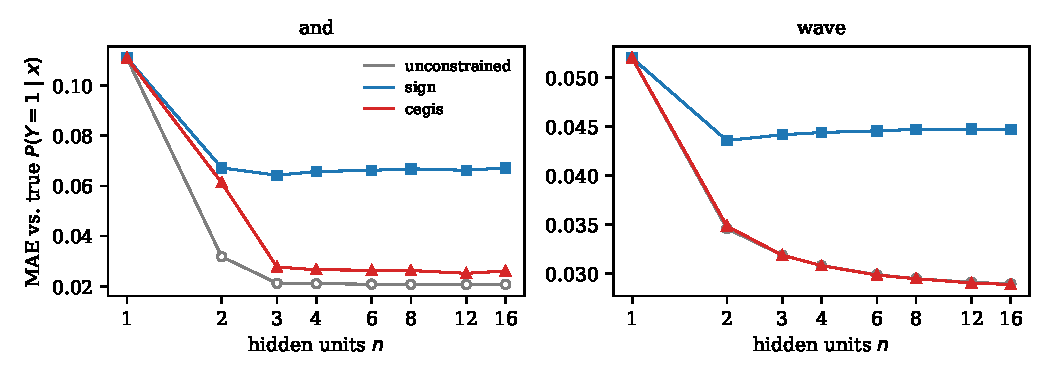
\includegraphics[width=0.9\textwidth]{figures/fig_capacity.pdf}}{\fbox{figure \pend}}
\caption{Error against the true probability versus the number of hidden units $n$, for the ``and'' target and the
``wave'' target $\sig(6(x_1+x_2)-6+1.5\sin(3(x_1-x_2)))$, which has no min/max structure. One network per size, trained
on the same 2000 samples (best of three initialisations, no model selection). Grey: unconstrained; blue: sign
constraints; red: cegis. Filled markers: certified by \cref{alg:bb}; open: counterexample found. With the sign
constraint the error stops decreasing after two units; cegis networks keep improving and are certified at every size,
about 0.005 above the (non-monotone) unconstrained networks on ``and'' and equal to them on ``wave''.}\label{fig:capacity}
\end{figure*}

% =====================================================================================================
\section{Gradients of the gains}\label{sup:gradients}
Write $a_j=\sig(z_j)$, $\sig_j'=a_j(1-a_j)$, $\sig_j''=\sig_j'(1-2a_j)$, $o=\sig(z_o)$, $\sig_o'=o(1-o)$,
$\sig_o''=\sig_o'(1-2o)$ and $u_i=\sum_jv_j\sig_j'W_{ji}$, so that $g_i=\sig_o'u_i$ (Lemma~\ref{M-lem:gain}). Then, for
$k=1,\dots,n$ and $l=1,\dots,p$,
\begin{align*}
\frac{\partial g_i}{\partial W_{kl}}&=\sig_o''\,v_k\sig_k'x_l\,u_i+\sig_o'\bigl(v_k\sig_k''x_lW_{ki}+v_k\sig_k'\,[i=l]\bigr),\\
\frac{\partial g_i}{\partial b_k}&=\sig_o''\,v_k\sig_k'\,u_i+\sig_o'\,v_k\sig_k''W_{ki},\\
\frac{\partial g_i}{\partial v_k}&=\sig_o''\,a_k\,u_i+\sig_o'\,\sig_k'W_{ki},\\
\frac{\partial g_i}{\partial c}&=\sig_o''\,u_i ,
\end{align*}
where $[i=l]$ is 1 if $i=l$ and 0 otherwise. SLSQP therefore receives exact constraint Jacobians instead of finite
differences. These expressions are checked against finite differences in the test suite of the code.

% =====================================================================================================
\section{Signal vectors and synthetic targets}\label{sup:signals}
\begin{table}[H]\centering\small
\caption{Expected gain signs. $+$: $P(Y=1\mid x)$ non-decreasing in the input; $-$: non-increasing; $0$: unconstrained.
The signs of the five UCI datasets were derived from domain knowledge; those of the benchmarks are the ones used in the
literature \citep{Liu2020,Sivaraman2020,Runje2023}.}\label{tab:signals}
\begin{tabular}{lp{0.82\textwidth}}\toprule
ID & Inputs (sign) \\\midrule
ALG & temperature ($+$), relative humidity ($-$), wind speed (0), rain ($-$), FFMC, DMC, DC, ISI, BUI, FWI ($+$) \\
BCO & clump thickness, uniformity of cell size, uniformity of cell shape, marginal adhesion, single epithelial cell size,
bare nuclei, bland chromatin, normal nucleoli, mitoses (all $+$) \\
BCD & mean, standard error and worst value of radius, texture, perimeter, area, smoothness, compactness, concavity,
concave points and symmetry ($+$); fractal dimension (0) \\
HF & age ($+$), anaemia ($+$), creatinine phosphokinase (0), diabetes (0), ejection fraction ($-$), high blood pressure
($+$), platelets (0), serum creatinine ($+$), serum sodium ($-$), sex (0), smoking (0), follow-up time ($-$) \\
PIM & pregnancies ($+$), glucose ($+$), blood pressure (0), skin thickness ($+$), insulin (0), BMI ($+$), diabetes
pedigree function ($+$), age ($+$) \\
HD & resting blood pressure ($+$), serum cholesterol ($+$); the other eleven inputs (0) \\
COM & prior adult convictions, juvenile felonies, juvenile misdemeanours, other juvenile counts ($+$); age, race and sex
indicators (0) \\
LOAN & credit score, length of employment, annual income ($-$); public-record bankruptcies, debt-to-income ratio ($+$);
23 other inputs (0) \todo{confirm the order of the first five features in the release} \\
\bottomrule\end{tabular}
\end{table}

\begin{table}[H]\centering\small
\caption{Synthetic targets, $P(Y=1\mid x)=\sig(\cdot)$ with $x$ uniform on $[0,1]^p$ and 2000 samples each. The minimum
and maximum targets favour Min-Max networks, whose functional form is a maximum of minima of hyperplanes; the product and
wave targets do not. The gains of ``wave'' stay between 1.5 and 10.5, but its natural representation uses the
non-monotone ridge $\sin(3(x_1-x_2))$.}\label{tab:synthdef}
\begin{tabular}{lll}\toprule
Name & Logit & Signs \\\midrule
and & $12(\min\{x_1,x_2\}-0.45)$ & $(+,+)$ \\
or & $12(\max\{x_1,x_2\}-0.55)$ & $(+,+)$ \\
prod & $12(x_1x_2-0.25)$ & $(+,+)$ \\
and3 & $12(\min\{x_1,x_2,x_3\}-0.35)$ & $(+,+,+)$ \\
andfree & $12(\min\{x_1,x_2\}-0.45)+1.5\sin(2\pi x_3)$ & $(+,+,0)$ \\
andneg & $12(\min\{x_1,1-x_2\}-0.45)$ & $(+,-)$ \\
wave & $6(x_1+x_2)-6+1.5\sin\bigl(3(x_1-x_2)\bigr)$ & $(+,+)$ \\
\bottomrule\end{tabular}
\end{table}

% =====================================================================================================
\section{Dynamic cross-validation}\label{sup:dcv}
\Cref{alg:dcv} states the selection procedure of Section~\ref{M-sec:dcv}.

\begin{algorithm}[H]
\caption{Dynamic cross-validation (DCV) inside a training set $T$.}\label{alg:dcv}
\begin{algorithmic}[1]
\State split $T$ into $K$ stratified folds $(T_k^{\mathrm{tr}},T_k^{\mathrm{va}})$; initialise one model $M_k$ per fold on $T_k^{\mathrm{tr}}$
\State $J^\ast\gets\infty$, $w\gets0$
\For{$n=1,2,\dots,n_{\max}$}
  \For{$k=1,\dots,K$} \State $M_k\gets$ constructive step $n$ of $M_k$ on $T_k^{\mathrm{tr}}$ (warm start from $M_k$ at $n-1$ if the method reuses weights) \EndFor
  \State $L_k(n)\gets\mathrm{BCE}\bigl(M_k;T_k^{\mathrm{va}}\bigr)$, $J(n)\gets\sum_k L_k(n)$ \ ($J(n)=\infty$ if some $M_k$ is infeasible)
  \If{$J(n)<J^\ast$} $J^\ast\gets J(n)$, $n^\ast\gets n$, $w\gets0$ \Else\ $w\gets w+1$; \textbf{if} $w=$ patience \textbf{break} \EndIf
\EndFor
\State $n^\ast_{1\mathrm{SE}}\gets\min\{n: J(n)\le J^\ast+\sqrt K\,\mathrm{sd}_k(L_k(n^\ast))\}$ \Comment{one-standard-error rule}
\State \Return networks retrained on $T$ with $n^\ast$ (DCV) and $n^\ast_{1\mathrm{SE}}$ (DCV-1SE) units
\end{algorithmic}
\end{algorithm}

% =====================================================================================================
\section{Settings and hyper-parameter grids}\label{sup:settings}
\begin{table}[H]\centering\small
\caption{Settings of the constructive networks (all experiments unless stated otherwise).}\label{tab:settings}
\begin{tabular}{@{}lp{0.62\textwidth}@{}}\toprule
Setting & Value \\\midrule
Maximum size, patience & 300 units, 30 steps (unconstrained); 50 units, 15 steps (constrained) \\
Prior precision & $\lambda_0=0.3$ in \eqref{M-eq:loss} \\
Optimisers & L-BFGS (unconstrained) and SLSQP (constrained, started from the unconstrained optimum), at most 1000 iterations; constraint tolerance $10^{-6}$ \\
Constraint margins & $\varepsilon_m=0.05$ (mean, at most 1000 random training points); $\varepsilon_p=10^{-3}$ (anchor, cegis) \\
Anchors & ten $k$-means centres, plus counterexamples (cegis) \\
Restarts & $R=100$ random restarts of an infeasible step \\
Initialisations & one per step on real data; best of three by training objective on synthetic data \\
cegis & $R_{\mathrm{cex}}=10$ counterexample rounds, adversarial search from 16 starting points; $R_{\mathrm{rep}}=20$ repairs \\
Certificate & $2\times10^5$ boxes (input space); 3000 linear programs (pre-activation space) \\
Selection & stratified 80/20 hold-out (validation MCC) or DCV with $K=4$ (summed cross-entropy); one-hour budget per selection loop \\
ELM & ReLU hidden units, weights and biases $U(-1,1)$, output bias; ELM-C: hidden weights of constrained inputs drawn with the prescribed sign (sign and cegis modes) \\
\bottomrule\end{tabular}
\end{table}

\begin{table}[H]\centering\small
\caption{Hyper-parameter grids of the baselines.}\label{tab:hyper}
\begin{tabular}{@{}lp{0.66\textwidth}@{}}\toprule
Method & Grid (selected by validation MCC; the chosen model is refitted on training + validation) \\\midrule
LR, LR-C & $L_2$ penalty $\in\{10^{-4},10^{-3},10^{-2},10^{-1}\}$; LR-C: coefficient signs bounded by $s$ \\
XGB(-C) & depth $\in\{2,3,4\}$, trees $\in\{100,300\}$, learning rate 0.05, subsample 0.9 \\
LGBM(-C) & leaves $\in\{4,8,16\}$, trees $\in\{100,300\}$, learning rate 0.05, subsample 0.9 \\
MLP & one hidden layer of $\{1,2,4,\dots,64\}$ logistic units \\
Min-Max & $K$ groups of $K$ hyperplanes, $K\in\{2,4,8\}$ \\
CMNN & width $\in\{8,16,32\}$, two monotone layers, ELU-based activations \\
LMN & width $\in\{16,32\}$, Lipschitz constant $\lambda\in\{2,8,32\}$, GroupSort \\
Min-Max, CMNN, LMN & Adam, learning rate $5\times10^{-3}$, batch 256, early stopping on the validation split (patience 50, at most 1000 epochs); refit for the selected number of epochs \\
\bottomrule\end{tabular}
\end{table}

\paragraph{Implementation}
Python with NumPy, SciPy (SLSQP, L-BFGS-B, HiGHS linear programs) and scikit-learn; the monotone baselines use PyTorch
and the authors' packages \texttt{mononet} and \texttt{monotonicnetworks}. In the code, the anchor and sign modes are
called \texttt{multi} and \texttt{global}. The closed-form gains, their gradients and the certificate are covered by unit
tests, including soundness checks of the certificate against dense sampling. Experiments ran on a 16-thread
workstation, one task per core.

% =====================================================================================================
\section{Additional results}\label{sup:more}
\IfFileExists{tables/main_mcc_full.tex}{\begin{table*}[!tbp]\centering
\caption{Test MCC on the real datasets, all methods: mean and, in parentheses, standard deviation over the outer folds. Conventions as in Table~\ref{M-tab:main_mcc} of the article; best value per dataset in bold; rank: average rank over the eight datasets.}
\label{tab:main_mcc_full}
\resizebox{\linewidth}{!}{\begin{tabular}{lllccccccccc}\toprule
Model & Constraint & Selection & ALG & BCO & BCD & HF & PIM & HD & COM & LOAN & Rank \\\midrule
\multicolumn{12}{l}{\textit{Certified SFNNs, counterexample-guided (this work)}} \\
WILCAR & cegis & DCV & 0.901\,{\scriptsize(0.06)} & 0.932\,{\scriptsize(0.03)} & 0.952\,{\scriptsize(0.03)} & 0.574\,{\scriptsize(0.11)} & 0.473\,{\scriptsize(0.07)} & 0.589\,{\scriptsize(0.12)} & 0.349\,{\scriptsize(0.03)} & 0.293\,{\scriptsize(0.02)} & 11.1 \\
WILCAR & cegis & hold-out & 0.906\,{\scriptsize(0.06)} & \textbf{0.937\,{\scriptsize(0.03)}} & 0.866\,{\scriptsize(0.26)} & 0.564\,{\scriptsize(0.10)} & 0.468\,{\scriptsize(0.07)} & 0.597\,{\scriptsize(0.12)} & 0.349\,{\scriptsize(0.03)} & 0.293\,{\scriptsize(0.02)} & 13.2 \\
RIXM & cegis & hold-out & 0.908\,{\scriptsize(0.06)} & 0.936\,{\scriptsize(0.03)} & 0.937\,{\scriptsize(0.05)} & 0.564\,{\scriptsize(0.11)} & 0.471\,{\scriptsize(0.07)} & 0.599\,{\scriptsize(0.12)} & 0.352\,{\scriptsize(0.03)} & 0.292\,{\scriptsize(0.02)} & 9.1 \\
\midrule
\multicolumn{12}{l}{\textit{SFNNs with sign constraints}} \\
WILCAR & sign & DCV & 0.899\,{\scriptsize(0.07)} & 0.929\,{\scriptsize(0.03)} & 0.953\,{\scriptsize(0.03)} & 0.574\,{\scriptsize(0.11)} & 0.471\,{\scriptsize(0.07)} & 0.589\,{\scriptsize(0.12)} & 0.350\,{\scriptsize(0.03)} & 0.292\,{\scriptsize(0.02)} & 12.2 \\
WILCAR & sign & hold-out & 0.909\,{\scriptsize(0.07)} & 0.932\,{\scriptsize(0.03)} & 0.916\,{\scriptsize(0.19)} & 0.564\,{\scriptsize(0.10)} & 0.470\,{\scriptsize(0.07)} & 0.597\,{\scriptsize(0.12)} & 0.348\,{\scriptsize(0.03)} & 0.286\,{\scriptsize(0.02)} & 15.4 \\
RIXM & sign & hold-out & 0.909\,{\scriptsize(0.07)} & 0.932\,{\scriptsize(0.03)} & \textbf{0.955\,{\scriptsize(0.03)}} & 0.562\,{\scriptsize(0.10)} & 0.468\,{\scriptsize(0.07)} & 0.601\,{\scriptsize(0.12)} & 0.350\,{\scriptsize(0.03)} & 0.291\,{\scriptsize(0.02)} & 11.2 \\
\midrule
\multicolumn{12}{l}{\textit{SFNNs with anchor constraints}} \\
WILCAR & anchor & DCV & 0.906\,{\scriptsize(0.06)} & 0.932\,{\scriptsize(0.03)} & 0.954\,{\scriptsize(0.03)} & 0.574\,{\scriptsize(0.11)} & 0.475\,{\scriptsize(0.07)} & 0.589\,{\scriptsize(0.12)} & 0.349\,{\scriptsize(0.03)} & 0.292\,{\scriptsize(0.02)} & 10.9 \\
WILCAR & anchor & hold-out & 0.906\,{\scriptsize(0.06)} & \textbf{0.937\,{\scriptsize(0.03)}} & 0.865\,{\scriptsize(0.26)} & 0.564\,{\scriptsize(0.10)} & 0.472\,{\scriptsize(0.07)} & 0.597\,{\scriptsize(0.12)} & 0.349\,{\scriptsize(0.03)} & 0.293\,{\scriptsize(0.02)} & 11.6 \\
RIXM & anchor & hold-out & 0.908\,{\scriptsize(0.06)} & 0.936\,{\scriptsize(0.03)} & 0.937\,{\scriptsize(0.05)} & 0.564\,{\scriptsize(0.11)} & 0.473\,{\scriptsize(0.07)} & 0.599\,{\scriptsize(0.12)} & 0.351\,{\scriptsize(0.03)} & 0.291\,{\scriptsize(0.02)} & 9.4 \\
\midrule
\multicolumn{12}{l}{\textit{SFNNs with the mean constraint}} \\
WILCAR & mean & DCV & 0.901\,{\scriptsize(0.06)} & 0.936\,{\scriptsize(0.03)} & 0.938\,{\scriptsize(0.04)} & 0.558\,{\scriptsize(0.10)} & \textbf{0.475\,{\scriptsize(0.07)}} & 0.589\,{\scriptsize(0.13)} & 0.350\,{\scriptsize(0.03)} & 0.293\,{\scriptsize(0.02)} & 10.9 \\
WILCAR & mean & hold-out & 0.907\,{\scriptsize(0.06)} & 0.935\,{\scriptsize(0.03)} & 0.896\,{\scriptsize(0.11)} & 0.556\,{\scriptsize(0.10)} & 0.471\,{\scriptsize(0.07)} & 0.598\,{\scriptsize(0.12)} & 0.351\,{\scriptsize(0.03)} & 0.292\,{\scriptsize(0.02)} & 12.4 \\
RIXM & mean & hold-out & 0.906\,{\scriptsize(0.06)} & 0.935\,{\scriptsize(0.03)} & 0.936\,{\scriptsize(0.04)} & 0.553\,{\scriptsize(0.10)} & 0.470\,{\scriptsize(0.07)} & 0.600\,{\scriptsize(0.12)} & 0.353\,{\scriptsize(0.03)} & 0.290\,{\scriptsize(0.02)} & 13.2 \\
\midrule
\multicolumn{12}{l}{\textit{Unconstrained SFNNs}} \\
WILCAR & none & DCV & 0.897\,{\scriptsize(0.07)} & 0.929\,{\scriptsize(0.03)} & 0.952\,{\scriptsize(0.03)} & 0.567\,{\scriptsize(0.12)} & 0.472\,{\scriptsize(0.07)} & 0.589\,{\scriptsize(0.12)} & 0.349\,{\scriptsize(0.03)} & 0.292\,{\scriptsize(0.02)} & 12.8 \\
WILCAR & none & hold-out & 0.907\,{\scriptsize(0.07)} & 0.931\,{\scriptsize(0.03)} & 0.953\,{\scriptsize(0.03)} & 0.562\,{\scriptsize(0.11)} & 0.469\,{\scriptsize(0.07)} & 0.598\,{\scriptsize(0.12)} & 0.348\,{\scriptsize(0.03)} & 0.290\,{\scriptsize(0.01)} & 14.2 \\
RIXM & none & hold-out & 0.907\,{\scriptsize(0.07)} & 0.931\,{\scriptsize(0.03)} & 0.954\,{\scriptsize(0.03)} & 0.563\,{\scriptsize(0.11)} & 0.473\,{\scriptsize(0.07)} & 0.599\,{\scriptsize(0.12)} & 0.351\,{\scriptsize(0.03)} & 0.294\,{\scriptsize(0.02)} & 8.8 \\
ELM & none & hold-out & 0.828\,{\scriptsize(0.07)} & 0.920\,{\scriptsize(0.03)} & 0.884\,{\scriptsize(0.06)} & 0.439\,{\scriptsize(0.14)} & 0.428\,{\scriptsize(0.10)} & 0.521\,{\scriptsize(0.17)} & 0.337\,{\scriptsize(0.03)} & 0.280\,{\scriptsize(0.02)} & 25.2 \\
MLP & none & hold-out & 0.868\,{\scriptsize(0.06)} & 0.934\,{\scriptsize(0.03)} & 0.949\,{\scriptsize(0.03)} & 0.556\,{\scriptsize(0.12)} & 0.427\,{\scriptsize(0.08)} & 0.585\,{\scriptsize(0.11)} & 0.344\,{\scriptsize(0.03)} & 0.291\,{\scriptsize(0.02)} & 18.5 \\
\midrule
\multicolumn{12}{l}{\textit{Monotone baselines}} \\
LR & sign & hold-out & 0.931\,{\scriptsize(0.07)} & 0.924\,{\scriptsize(0.03)} & 0.954\,{\scriptsize(0.03)} & 0.576\,{\scriptsize(0.12)} & 0.455\,{\scriptsize(0.07)} & 0.569\,{\scriptsize(0.15)} & 0.344\,{\scriptsize(0.03)} & 0.286\,{\scriptsize(0.02)} & 15.4 \\
XGBoost & monotone & hold-out & \textbf{0.967\,{\scriptsize(0.03)}} & 0.926\,{\scriptsize(0.04)} & 0.931\,{\scriptsize(0.03)} & 0.617\,{\scriptsize(0.12)} & 0.462\,{\scriptsize(0.07)} & 0.515\,{\scriptsize(0.11)} & 0.357\,{\scriptsize(0.02)} & \textbf{0.295\,{\scriptsize(0.02)}} & 11.2 \\
LightGBM & monotone & hold-out & 0.950\,{\scriptsize(0.05)} & 0.922\,{\scriptsize(0.04)} & 0.933\,{\scriptsize(0.03)} & 0.628\,{\scriptsize(0.11)} & 0.459\,{\scriptsize(0.09)} & 0.518\,{\scriptsize(0.12)} & 0.356\,{\scriptsize(0.02)} & 0.295\,{\scriptsize(0.02)} & 11.9 \\
Min-Max & structural & hold-out & 0.911\,{\scriptsize(0.07)} & 0.925\,{\scriptsize(0.03)} & 0.914\,{\scriptsize(0.04)} & 0.539\,{\scriptsize(0.10)} & 0.455\,{\scriptsize(0.08)} & 0.544\,{\scriptsize(0.14)} & 0.348\,{\scriptsize(0.03)} & 0.288\,{\scriptsize(0.02)} & 20.4 \\
CMNN & structural & hold-out & 0.937\,{\scriptsize(0.07)} & 0.927\,{\scriptsize(0.03)} & 0.947\,{\scriptsize(0.03)} & 0.562\,{\scriptsize(0.11)} & 0.466\,{\scriptsize(0.08)} & \textbf{0.610\,{\scriptsize(0.12)}} & 0.354\,{\scriptsize(0.03)} & 0.293\,{\scriptsize(0.02)} & 10.4 \\
LMN & structural & hold-out & 0.894\,{\scriptsize(0.07)} & 0.932\,{\scriptsize(0.03)} & 0.929\,{\scriptsize(0.05)} & 0.545\,{\scriptsize(0.12)} & 0.448\,{\scriptsize(0.07)} & 0.548\,{\scriptsize(0.14)} & 0.346\,{\scriptsize(0.03)} & 0.291\,{\scriptsize(0.02)} & 20.0 \\
\midrule
\multicolumn{12}{l}{\textit{Unconstrained baselines}} \\
LR & none & hold-out & 0.911\,{\scriptsize(0.07)} & 0.924\,{\scriptsize(0.03)} & 0.950\,{\scriptsize(0.03)} & 0.555\,{\scriptsize(0.13)} & 0.455\,{\scriptsize(0.07)} & 0.567\,{\scriptsize(0.15)} & 0.346\,{\scriptsize(0.02)} & 0.285\,{\scriptsize(0.02)} & 18.7 \\
XGBoost & none & hold-out & \textbf{0.967\,{\scriptsize(0.03)}} & 0.929\,{\scriptsize(0.03)} & 0.926\,{\scriptsize(0.02)} & \textbf{0.630\,{\scriptsize(0.11)}} & 0.449\,{\scriptsize(0.08)} & 0.523\,{\scriptsize(0.12)} & \textbf{0.357\,{\scriptsize(0.03)}} & 0.294\,{\scriptsize(0.02)} & 11.4 \\
LightGBM & none & hold-out & 0.947\,{\scriptsize(0.05)} & 0.935\,{\scriptsize(0.04)} & 0.927\,{\scriptsize(0.03)} & 0.610\,{\scriptsize(0.10)} & 0.469\,{\scriptsize(0.06)} & 0.518\,{\scriptsize(0.12)} & 0.354\,{\scriptsize(0.03)} & 0.291\,{\scriptsize(0.02)} & 11.4 \\
\bottomrule\end{tabular}}
\end{table*}}{}
\IfFileExists{tables/main_auc.tex}{\begin{table*}[t]\centering
\caption{Test AUC (mean and standard deviation over the outer folds; $5\times5$-fold nested cross-validation, $5\times2$ for COM and LOAN). $\star$: counterexample-guided constraints with branch-and-bound certificate (Section~\ref{sec:cegis}). Best value per dataset in bold; last column: average rank over the datasets with complete results (Friedman ranks).}
\label{tab:main_auc}
\resizebox{\textwidth}{!}{\begin{tabular}{lccccccccc}\toprule
Method & ALG & BCO & BCD & HF & PIM & HD & COM & LOAN & Rank \\\midrule
WILCAR-C$^{\star}$ (DCV-1SE) & -- & -- & -- & -- & -- & -- & -- & -- & -- \\
WILCAR-C$^{\star}$ (DCV) & -- & -- & -- & -- & -- & -- & -- & -- & -- \\
WILCAR-C$^{\star}$ & -- & -- & -- & -- & -- & -- & -- & -- & -- \\
RIXM-C$^{\star}$ & -- & -- & -- & -- & -- & -- & -- & -- & -- \\
\midrule
WILCAR-C (mean) & 0.992\,{\scriptsize(0.01)} & 0.996\,{\scriptsize(0.00)} & 0.979\,{\scriptsize(0.06)} & -- & -- & -- & -- & -- & -- \\
WILCAR-C (mean, DCV) & 0.992\,{\scriptsize(0.01)} & \textbf{0.996\,{\scriptsize(0.00)}} & -- & -- & -- & -- & -- & -- & -- \\
WILCAR (DCV-1SE) & -- & -- & -- & -- & -- & -- & -- & -- & -- \\
WILCAR (DCV) & 0.992\,{\scriptsize(0.01)} & 0.995\,{\scriptsize(0.00)} & \textbf{0.994\,{\scriptsize(0.01)}} & -- & -- & -- & -- & -- & -- \\
WILCAR & 0.993\,{\scriptsize(0.01)} & 0.996\,{\scriptsize(0.00)} & 0.994\,{\scriptsize(0.01)} & -- & -- & -- & -- & -- & -- \\
RIXM & 0.993\,{\scriptsize(0.01)} & 0.996\,{\scriptsize(0.00)} & -- & -- & -- & -- & -- & -- & -- \\
\midrule
ELM & 0.972\,{\scriptsize(0.02)} & 0.993\,{\scriptsize(0.00)} & -- & -- & -- & -- & -- & -- & -- \\
\midrule
MLP & 0.979\,{\scriptsize(0.02)} & 0.995\,{\scriptsize(0.00)} & -- & -- & -- & -- & -- & -- & -- \\
LR-C & 0.995\,{\scriptsize(0.01)} & 0.995\,{\scriptsize(0.00)} & -- & -- & -- & -- & -- & -- & -- \\
XGB-C & \textbf{0.998\,{\scriptsize(0.00)}} & 0.993\,{\scriptsize(0.00)} & -- & -- & -- & -- & -- & -- & -- \\
LGBM-C & 0.998\,{\scriptsize(0.00)} & 0.994\,{\scriptsize(0.00)} & -- & -- & -- & -- & -- & -- & -- \\
Min-Max & 0.990\,{\scriptsize(0.01)} & 0.994\,{\scriptsize(0.00)} & -- & -- & -- & -- & -- & -- & -- \\
CMNN & 0.994\,{\scriptsize(0.01)} & 0.995\,{\scriptsize(0.00)} & -- & -- & -- & -- & -- & -- & -- \\
LMN & 0.986\,{\scriptsize(0.02)} & 0.995\,{\scriptsize(0.00)} & -- & -- & -- & -- & -- & -- & -- \\
\bottomrule\end{tabular}}
\par\smallskip\footnotesize\textit{Pending runs: cegis}.
\end{table*}}{}
\IfFileExists{tables/main_brier.tex}{\begin{table*}[!tbp]\centering
\caption{Test Brier score on the real datasets (mean and, in parentheses, standard deviation over the outer folds). Rows, groups and conventions as in Table~\ref{M-tab:main_mcc} of the main article; rank over the datasets with complete results.}
\label{tab:main_brier}
\resizebox{\linewidth}{!}{\begin{tabular}{lllccccccccc}\toprule
Model & Constraint & Selection & ALG & BCO & BCD & HF & PIM & HD & COM & LOAN & Rank \\\midrule
\multicolumn{12}{l}{\textit{Certified SLFNs (this work)}} \\
WILCAR & cegis & DCV-1SE & -- & -- & -- & -- & -- & -- & -- & -- & -- \\
WILCAR & cegis & DCV & -- & -- & -- & -- & -- & -- & -- & -- & -- \\
WILCAR & cegis & hold-out & -- & -- & -- & -- & -- & -- & -- & -- & -- \\
RIXM & cegis & hold-out & -- & -- & -- & -- & -- & -- & -- & -- & -- \\
\midrule
\multicolumn{12}{l}{\textit{SLFNs with the average-gain constraint of \citet{Sa2026}}} \\
WILCAR & mean & DCV-1SE & -- & -- & -- & -- & -- & -- & -- & -- & -- \\
WILCAR & mean & DCV & 0.046\,{\scriptsize(0.02)} & \textbf{0.023\,{\scriptsize(0.01)}} & -- & -- & -- & -- & -- & -- & 8.0 \\
WILCAR & mean & hold-out & 0.046\,{\scriptsize(0.01)} & 0.023\,{\scriptsize(0.01)} & 0.045\,{\scriptsize(0.05)} & -- & -- & -- & -- & -- & 7.5 \\
RIXM & mean & hold-out & 0.046\,{\scriptsize(0.01)} & 0.023\,{\scriptsize(0.01)} & -- & -- & -- & -- & -- & -- & 7.5 \\
\midrule
\multicolumn{12}{l}{\textit{Unconstrained SLFNs}} \\
WILCAR & none & DCV-1SE & -- & -- & -- & -- & -- & -- & -- & -- & -- \\
WILCAR & none & DCV & 0.046\,{\scriptsize(0.01)} & 0.023\,{\scriptsize(0.01)} & 0.023\,{\scriptsize(0.01)} & -- & -- & -- & -- & -- & 8.5 \\
WILCAR & none & hold-out & 0.045\,{\scriptsize(0.01)} & 0.023\,{\scriptsize(0.01)} & 0.022\,{\scriptsize(0.01)} & -- & -- & -- & -- & -- & 7.0 \\
RIXM & none & hold-out & 0.045\,{\scriptsize(0.01)} & 0.023\,{\scriptsize(0.01)} & -- & -- & -- & -- & -- & -- & 7.0 \\
ELM & none & hold-out & 0.075\,{\scriptsize(0.03)} & 0.033\,{\scriptsize(0.01)} & -- & -- & -- & -- & -- & -- & 17.0 \\
MLP & none & hold-out & 0.061\,{\scriptsize(0.03)} & 0.027\,{\scriptsize(0.01)} & -- & -- & -- & -- & -- & -- & 16.0 \\
\midrule
\multicolumn{12}{l}{\textit{Monotone baselines}} \\
LR & sign & hold-out & 0.033\,{\scriptsize(0.02)} & 0.025\,{\scriptsize(0.01)} & -- & -- & -- & -- & -- & -- & 7.5 \\
XGBoost & monotone & hold-out & \textbf{0.014\,{\scriptsize(0.01)}} & 0.026\,{\scriptsize(0.01)} & -- & -- & -- & -- & -- & -- & 7.0 \\
LightGBM & monotone & hold-out & 0.019\,{\scriptsize(0.02)} & 0.027\,{\scriptsize(0.01)} & -- & -- & -- & -- & -- & -- & 9.0 \\
Min-Max & structural & hold-out & 0.036\,{\scriptsize(0.02)} & 0.025\,{\scriptsize(0.01)} & -- & -- & -- & -- & -- & -- & 9.0 \\
CMNN & structural & hold-out & 0.028\,{\scriptsize(0.02)} & 0.024\,{\scriptsize(0.01)} & -- & -- & -- & -- & -- & -- & 6.0 \\
LMN & structural & hold-out & 0.046\,{\scriptsize(0.03)} & 0.025\,{\scriptsize(0.01)} & -- & -- & -- & -- & -- & -- & 11.0 \\
\midrule
\multicolumn{12}{l}{\textit{Unconstrained baselines}} \\
LR & none & hold-out & 0.038\,{\scriptsize(0.02)} & 0.025\,{\scriptsize(0.01)} & -- & -- & -- & -- & -- & -- & 9.0 \\
XGBoost & none & hold-out & 0.014\,{\scriptsize(0.01)} & 0.026\,{\scriptsize(0.01)} & -- & -- & -- & -- & -- & -- & 8.0 \\
LightGBM & none & hold-out & 0.022\,{\scriptsize(0.02)} & 0.026\,{\scriptsize(0.01)} & -- & -- & -- & -- & -- & -- & 8.0 \\
\bottomrule\end{tabular}}
\par\smallskip\footnotesize\textit{Datasets complete so far: ALG, BCO. Pending campaigns: cegis.}
\end{table*}}{}
\IfFileExists{tables/size.tex}{\begin{table*}[!tbp]\centering
\caption{Selected number of hidden units $n^\ast$ and, in parentheses, time per outer fold (selection, refit and certificate), means over the outer folds. DCV: size minimising the summed validation cross-entropy; DCV-1SE: smallest size within one standard error of that minimum.}
\label{tab:size}
\resizebox{\linewidth}{!}{\begin{tabular}{lllcccccccc}\toprule
Model & Constraint & Selection & ALG & BCO & BCD & HF & PIM & HD & COM & LOAN \\\midrule
WILCAR & none & hold-out & 1.1\,{\scriptsize(1\,s)} & 2.0\,{\scriptsize(1\,s)} & 1.1\,{\scriptsize(1\,s)} & -- & -- & -- & -- & -- \\
WILCAR & none & DCV & 149.5\,{\scriptsize(25\,s)} & 18.6\,{\scriptsize(8\,s)} & 71.0\,{\scriptsize(23\,s)} & -- & -- & -- & -- & -- \\
WILCAR & none & DCV-1SE & -- & -- & -- & -- & -- & -- & -- & -- \\
RIXM & none & hold-out & 1.1\,{\scriptsize(3\,s)} & 2.0\,{\scriptsize(3\,s)} & -- & -- & -- & -- & -- & -- \\
WILCAR & mean & hold-out & 1.0\,{\scriptsize(5\,s)} & 1.7\,{\scriptsize(7\,s)} & 1.7\,{\scriptsize(867\,s)} & -- & -- & -- & -- & -- \\
WILCAR & mean & DCV & 33.6\,{\scriptsize(77\,s)} & 20.6\,{\scriptsize(111\,s)} & -- & -- & -- & -- & -- & -- \\
RIXM & mean & hold-out & 1.0\,{\scriptsize(3\,s)} & 1.7\,{\scriptsize(10\,s)} & -- & -- & -- & -- & -- & -- \\
WILCAR & cegis & hold-out & -- & -- & -- & -- & -- & -- & -- & -- \\
WILCAR & cegis & DCV & -- & -- & -- & -- & -- & -- & -- & -- \\
WILCAR & cegis & DCV-1SE & -- & -- & -- & -- & -- & -- & -- & -- \\
RIXM & cegis & hold-out & -- & -- & -- & -- & -- & -- & -- & -- \\
\bottomrule\end{tabular}}\end{table*}}{}

\begin{figure}[H]\centering
\IfFileExists{figures/fig_cd.pdf}{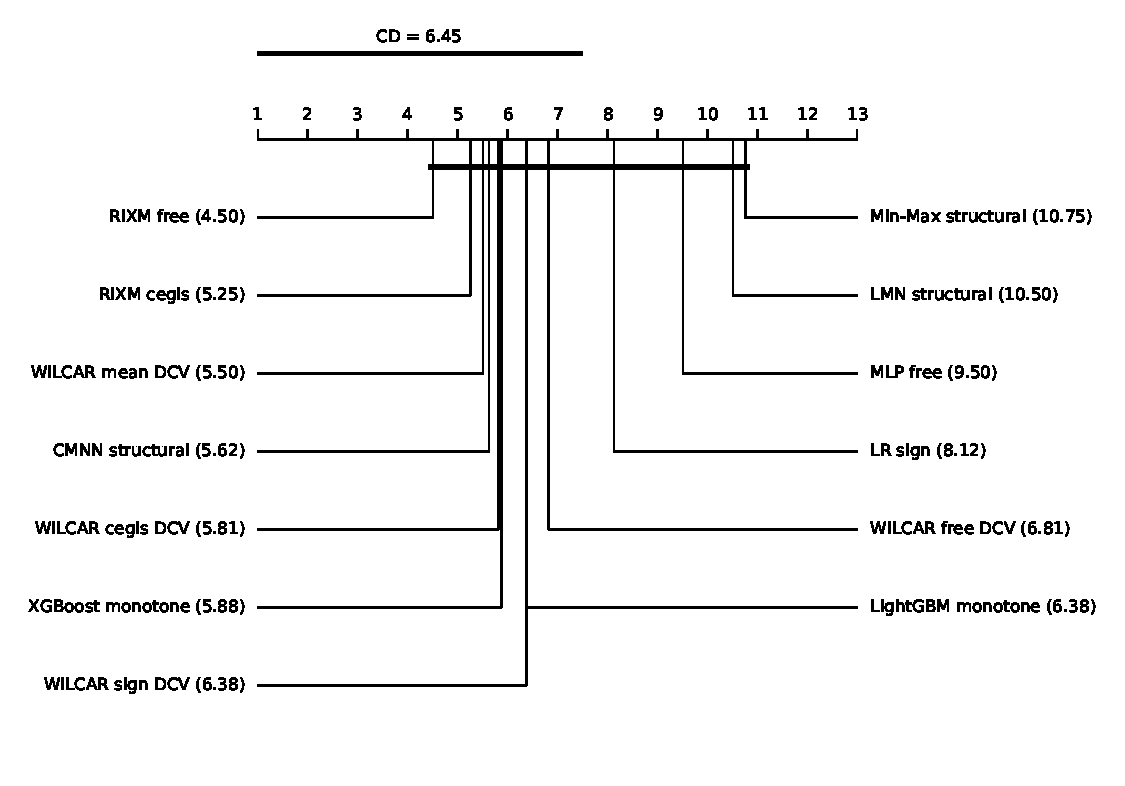
\includegraphics[width=0.9\textwidth]{figures/fig_cd.pdf}}{\fbox{critical-difference diagram \pend}}
\caption{Average MCC ranks of the methods of Table~\ref{M-tab:main_mcc} over the eight datasets and Nemenyi critical
difference ($\alpha=0.05$); methods joined by a thick bar are not significantly different.}\label{fig:cd}
\end{figure}

\bibliographystyle{elsarticle-harv}
\bibliography{refs}

\end{document}
